%% Single-site effective Hamiltonian
%
% The single-site effective Hamiltonian, applied to the center: H_eff AC.
%
% The state is in mixed canonical form with its center AC on this site, so
% everything to the left of it contracts into L and everything to the right
% into R. One-site DMRG finds the lowest eigenvector of this operator, one-site
% TDVP integrates i dAC/dt = H_eff AC with it, VUMPS solves for its fixed
% point; the picture is the same in all three, which is why it is named for
% what it is rather than for any of them.
%
% The bra layer is empty, and its three indices are the free ones -- the
% result is a tensor shaped like AC. Each ends at the border the tensor in that
% slot would have.
\documentclass[border=4pt]{standalone}
\usepackage{amsmath,amssymb}
\usepackage{tikz-tensors}
\input{notation}
\begin{document}
\begin{tikzpicture}
  \tnstack[left=$L$, right=$R$]{H}{1}{ket, op, bra}
  \tnlayer{H}{ket}{center/$A_C$}
  \tnlayer{H}{op}{mpo/$W$}
  \tnconnect{H}
  \tnopen[label=$\sigma$]{down}{H-op-1}
  \tnput[below]{H-bra-left}{$a$}
  \tnput[below]{H-bra-right}{$b$}
\end{tikzpicture}
\end{document}
